\begin{figure}[!t]
  \center {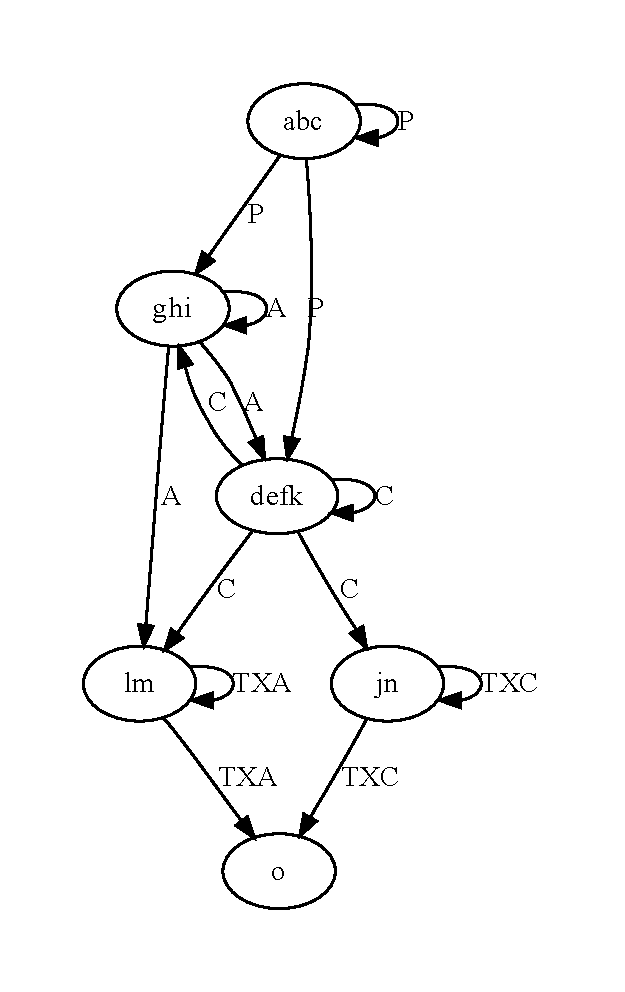
\includegraphics[scale=.6]{img/2pc_k1_noinv.pdf}}
  \caption{A representation derived for a synthetic two-phase commit
    trace using GK-Tail with k=1 and with temporal invariant checking
    disabled. States are labeled with letters whose combination
    indicates a particular merge of single letter states of the FSM in
    Figure~\ref{fig:2pc_k2_inv}.}
\label{fig:2pc_k1_noinv}
\end{figure}

\begin{figure}[!t]
  \center {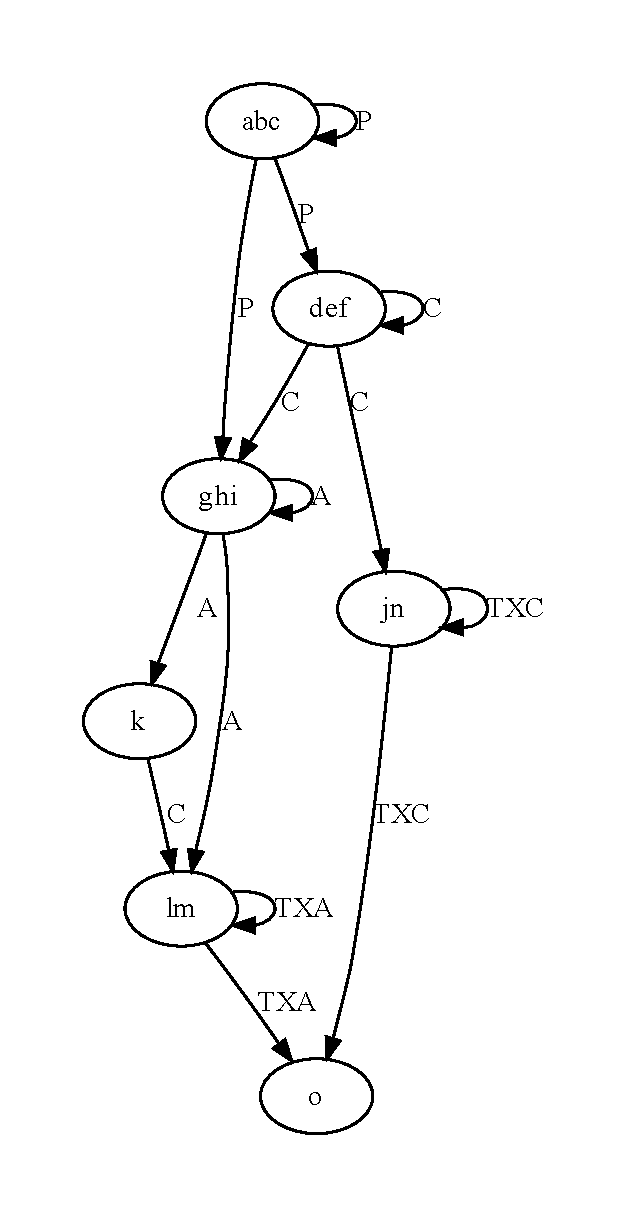
\includegraphics[scale=.6]{img/2pc_k1_inv.pdf}}
  \caption{A representation derived for a synthetic two-phase commit
    trace using GK-Tail with k=1 and with temporal invariant checking
    enabled. States are labeled with letters whose combination
    indicates a particular merge of single letter states of the FSM in
    Figure~\ref{fig:2pc_k2_inv}.}
  \label{fig:2pc_k1_inv}
\end{figure}

\begin{figure}[!t]
  \center {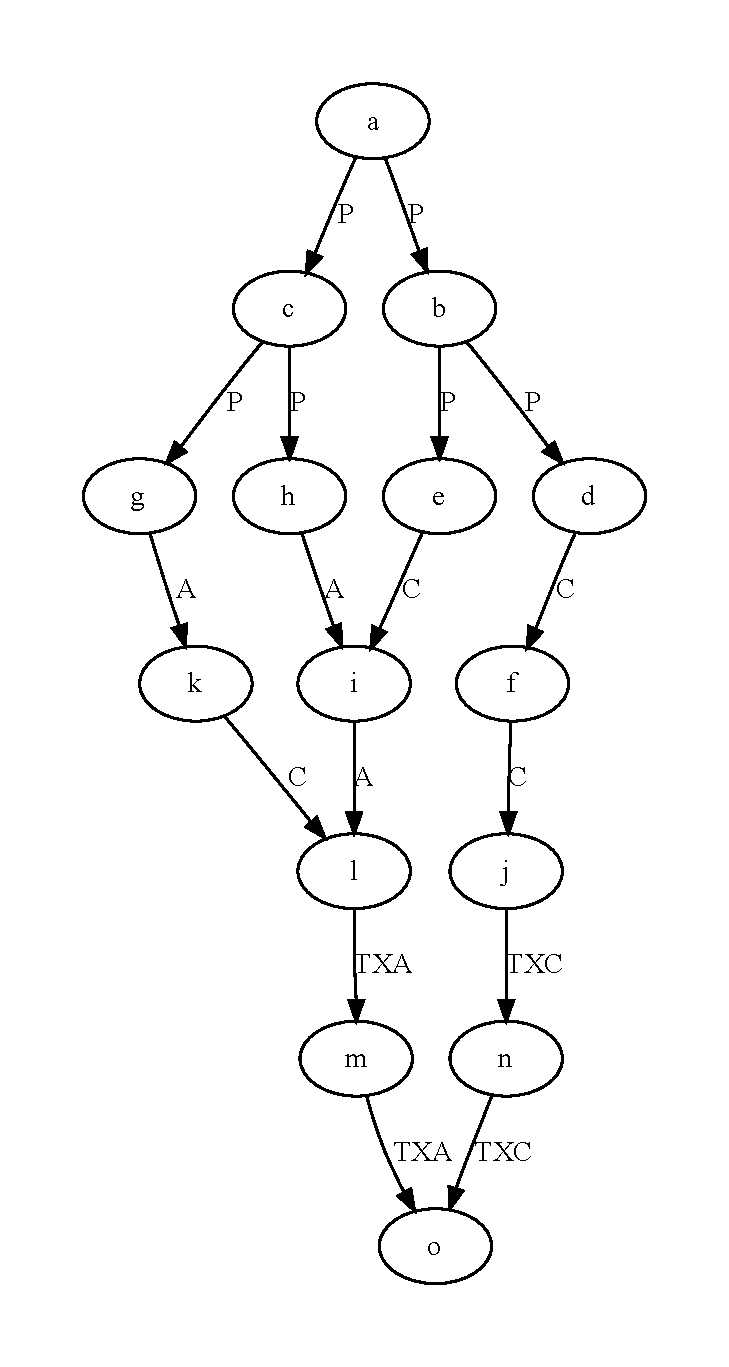
\includegraphics[scale=.6]{img/2pc_k2_inv.pdf}}
  \caption{A representation derived for a synthetic two-phase commit
    trace using GK-Tail with k=2 and with temporal invariant checking
    enabled.}
  \label{fig:2pc_k2_inv}
\end{figure}


%%%%%%%%%%%%%%%%%%%%%%%%%%%%%%%%%%%%%%%%%%%%%%%%%%%%%%%%%%%%%%%%%%%%%
\section{Evaluation}
\label{sec:evaluation}
%%%%%%%%%%%%%%%%%%%%%%%%%%%%%%%%%%%%%%%%%%%%%%%%%%%%%%%%%%%%%%%%%%%%%

We implemented Synoptic in Java. The core of the system (excluding
tests) is implemented in approximately 3,800 lines of
code. Internally, the GK-Tail and the Bikon algorithms use the
system-state and the relational representations
respectively. Internally, the decision engine uses the relational
representation -- GK-Tail graphs are converted every time it uses the
decision engine. We use dot~\cite{dot} to generate the visual
representations of Synoptic output. As a side-note, for the
non-synthetic systems we evaluate in this section, we additionally
augment the edges in the system-state representations with a count of
the number of messages observed in the trace along that transition.

In the remainder of this section we evaluate our work by applying
Synoptic to a variety of distributed systems and protocols. We start
off by using Synoptic to learn about the Twitter API and in this
context consider the difficulty of modifying an existing system to log
messages. We then elucidate some of the properties of our two
algorithms by applying Synoptic to synthetic traces of the two-phase
commit protocol. Next, we use Synoptic on traces of the Network File
System to illustrate the importance of choosing appropriate message
partitions. We then report on a user study with a system developer in
which Synoptic was applied to traces of a system intended for findings
the reverse traceroute between two internet hosts. We conclude this
section by evaluating Synoptic's performance across a variety of
dimensions.

%run the program on selected distributed systems, including
%Hadoop~\cite{Hadoop} and Harmony~\cite{Harmony}. The evaluation
%criteria of the representation output by Synoptic properties will
%include conciseness information content, and usefulness.

\subsection{Modifying Existing Systems for Logging}

\begin{figure}[!t]
\small
\begin{verbatim}
message SynopticMessage {
  required string src = 1;
  required string dst = 2;
  required int64 tstamp = 3;
  required string message_type = 4;
  required bytes system_message = 5;
    //system_message is a ByteStream
    //encoding of a protobuf format
    //message for the system in question
}
\end{verbatim}                                 
\caption{Protobuf format of a wrapped captured message.}
\label{fig:protobuf_example}
\end{figure}

One of the questions we wanted to answer is how difficult is to
instrument an existing system to output traces in a form that Synoptic
can process automatically? To provide an initial answer to this
question we designed a protobuf message specification
interface~\cite{protobuf} to Synoptic, and instrumented an existing
system to use it.

\subsubsection{Leveraging protobuf message specifications}

Because manual system instrumentation is necessary, we decided to
leverage protobuf~\cite{protobuf} message specifications to simplify
our task. This specification captures all the message fields and their
types. The availability of a protobuf specification may enable future
structural analysis of the messages observed, and simplifies
serialization and deserialization of system messages to and from a
trace file. These specifications also provide a natural way to
distinguish messages according to their type.

% Synoptic additionally needs the  that the user specifies the fields of
% the protobuf specifications that should be used for structural
% invariant mining.

We manually wrap all captured messages into a custom message type, the
structure of which is depicted in
Figure~\ref{fig:protobuf_example}. This message specification augments
captured messages with meta-information, such as the source and
destination addresses, and a message timestamp. The procedure of
formulating this specification must be manually repeated for each
system that we study.

We then combine the protobuf wrapper with a Tracer class which
provides static methods for logging messages in a system.  With these
two frameworks in place, instrumentation of existing systems,
especially those using protobuf formatted messages, is
straightforward.

\subsubsection{Twitter Java library evaluation}

We apply Synoptic to traces generated by the Java wrapper of the
Twitter API~\cite{JavaTwitterAPI}. Modification of the Java Twitter
API required us to add calls to Tracer.log() at two locations in the
code where protobuf messages were about to be converted to an outgoing
on-the-wire format. In addition we added this call to where incoming
messages are processed. In total we added \textbf{three} lines of code
to an existing system to automate the processing of its message logs
with Synoptic.

% Unlike the other systems we evaluate, we evaluate this system so as to
% understand the difficulty of modifying existing code to output traces
% in a form that Synoptic can process automatically.

We built a basic Twitter client that successfully performed a range of
Twitter operations using the instrumented Twitter API, logging all the
messages sent and received from the Twitter server. These messages were
then processed by Synoptic automatically. Figure~\ref{fig:twitter_api}
(in the Appendix) illustrates the resulting collection of FSMs
generated by Bikon (and then converted into system-state
representation). The GK-Tail algorithm yielded a similar
representation, except that the final states of all the FSMs were
merged into a single state at the very end. We think the resulting
representation is an intuitive means of documenting the Twitter
API. Though the original system is not complex, this example
illustrates that it is straightforward to modify an existing systems
to log messages for automated analysis with Synoptic.

\subsection{Two-Phase Commit Protocol}

We evaluated our framework on synthetic traces of a three-node
two-phase commit protocol (with one node acting as the transaction
manager). We used a synthetic trace to understand the impact of our
choices on the design of GK-Tail and Bikon algorithms.

\subsubsection{GK-Tail}

The graph generated with GK-Tail with $k=1$ and with disabled
invariant detection is depicted in Figure
\ref{fig:2pc_k1_noinv}. Considering that this representation can
generate an invalid trace containing both, (A)bort and (TX-C)ommit, it
is clear that this is not a good representation of the traces. The
representation also contains self-loops, and thus allows for behavior
that is valid but which was not observed in the input traces.

The same input was also processed with $k=1$ and with invariant
detection enabled and is depicted in Figure~\ref{fig:2pc_k1_inv}. The
spurious trace is gone, since the crucial invariant was enforced by
the decision engine. However, the FSM contains self-loops, and thus
allows for an unbounded number of (A)borts and (C)ommits to occur
before the transaction is eventually finished. This does not capture
the important property that only two nodes participate in the
protocol.

The most concise representation of the graph is obtained with $k=2$
and is shown in Figure~\ref{fig:2pc_k2_inv}. In this case, the
invariant detection does \emph{not} alter the output. This is because
the temporal invariant span is two, and $k=2$ guarantees that traces
up to this length are preserved. The significant improvement over
Figure~\ref{fig:2pc_k1_inv} is the absence of self-loops. Although the
graph clearly shows that no more than two commits can occur, it misses
the opportunity to merge states g, h, e, and d.

Although checking temporal invariants does not alter the final
representation for $k=2$, it is important to note that choosing the
right value of $k$ is difficult without deep understanding of the
system. Additionally, our results indicate that the choice of $k$ is
crucial even in the presence of invariants. On the other hand we have
shown that small values of $k$ in combination with invariant detection
lead to smaller and - more importantly - correct, graph representation
for our two-phase commit traces.

% \subsection{Small and Interesting Distributed Systems}

% We plan to drive the development of Synoptic by applying it to
% interesting networked test program. Here is a set of such programs that
% we think are appropriate for this purpose:

% \begin{itemize}

% \item A \texttt{ping-pong} system which consist of two nodes each
%   oscillating between two states. It will be the job of our tool to
%   infer these state sequences.

% \item A \texttt{demux} node, which forwards incoming packets to 
% different nodes according to properties of the payload. We want to 
% infer the relation between payload and forwarding destination.

% \item A storage and retrieval system. The goal of our tool here may be
%   to infer the constraint of a retrieve request always returning a
%   modified result after a store request.

% \item Other ideas include more complicated client-server systems where
%   concurrent client access may force the inference engine to consider
%   how to represent synchronization and concurrency.

% \end{itemize}

\subsubsection{Bikon}
\label{section:bisim-eval}

Bikon is able to produce the trace in Figure \ref{fig:2pc_k1_inv} as
well. The trace in Figure \ref{fig:2pc_k2_inv} is out of reach, and we
experienced the same problems with self-loops. We feel that the
strength of Bikon lies in its ability to consider statistics,
i.e. whether a node should be split could potentially made dependent
on the properties of the other nodes in that partition. This is a
direction we intend to pursue in our future work.

\begin{figure*}[!t]
  \center {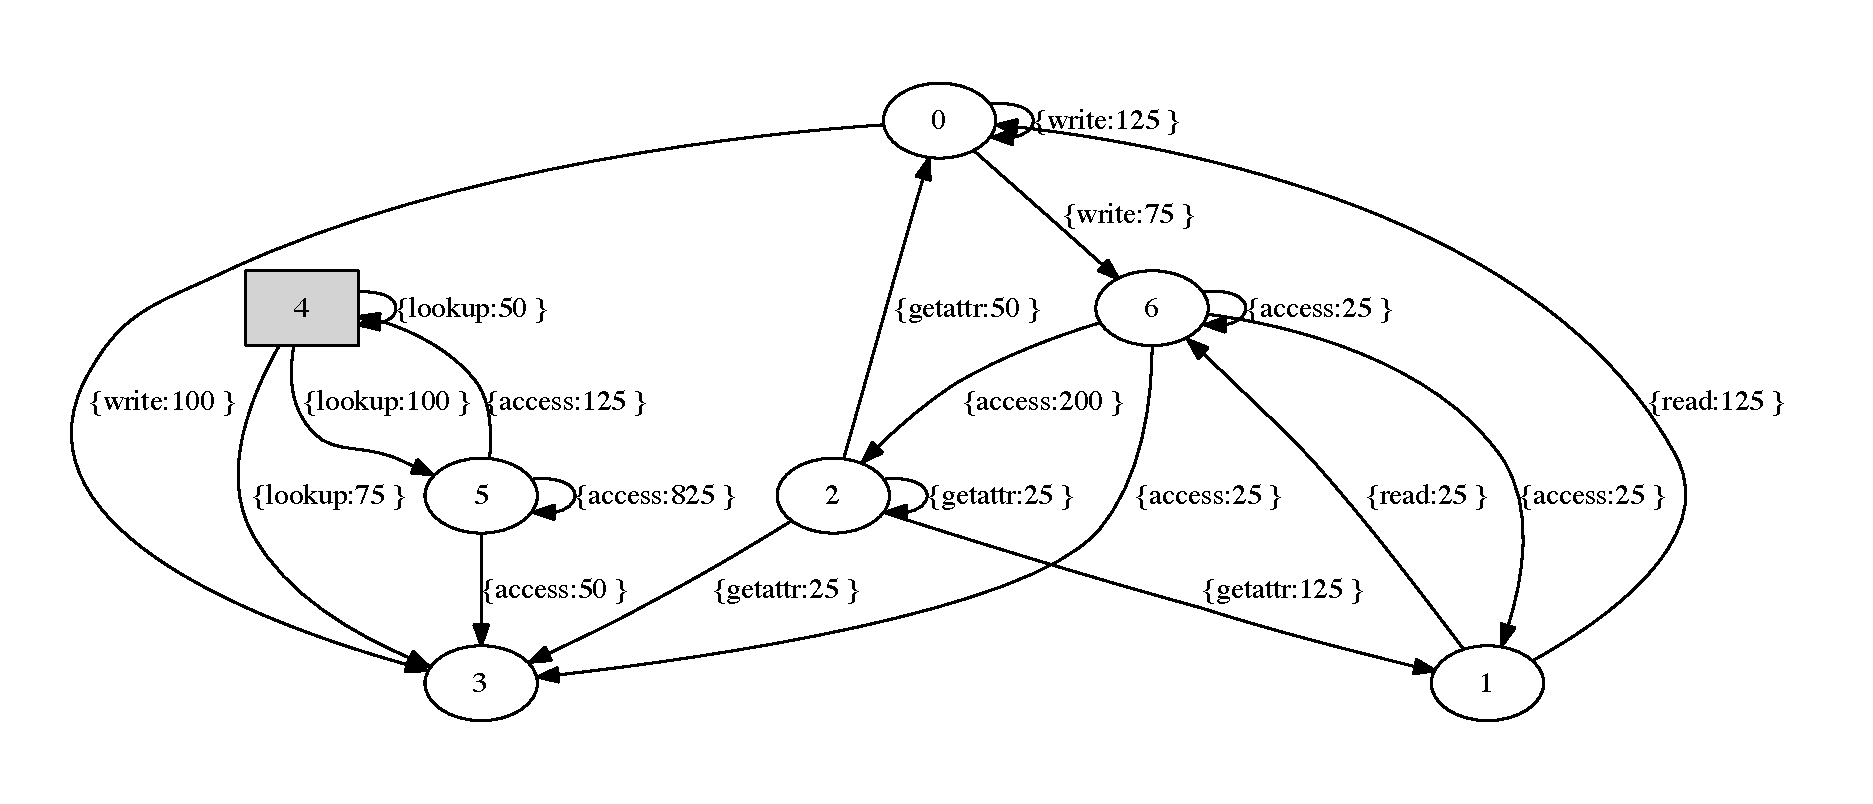
\includegraphics[scale=.6]{img/nfs_by_file.pdf}}
  \caption{A representation derived for 2K lines of NFS traces
    partitioned by file ID. The rectangular grey node indicates the
    start state. Generated using GK-Tail with k = 1.}
  \label{fig:nfs_1}
\end{figure*}

\subsection{Network File System}

We applied Synoptic to a set of Network File System collected by the
Self Organizing Storage project~\cite{SOS03} and evaluated the
resulting representations. The contribution of this evaluation was
two-fold. This set of real-world traces exposed the limitations of our
framework as well as demonstrated the importance of choosing an
intelligent partitioning strategy.

Initially, we applied our framework to NFS traces with no
partitioning. NFS~\cite{NFSv3RFC} is a stateless protocol (see
section~1.6 in~\cite{NFSv3RFC}) which implies that a large enough
input trace without any partitioning results in a representation that
is a fully connected graph. This happens because in a stateless
protocol it is possible for any message to follow any other
message. Thus, in the absence of temporal invariants in the trace,
this demonstrates a fundamental limitation of our summarization
approach.

We then considered the same traces partitioned by accessed file
ID. This produces a set of traces with each trace representing
successive NFS operations performed against a single file. While NFS
is a stateless protocol, in practice interaction with a particular
file is \emph{not} stateless. The representation produced by Synoptic
clearly shows this, as seen in Figure~\ref{fig:nfs_1}. We believe that
this representation may help to answer a variety of questions
concerning file access patterns in NFS (e.g. which files are only
read, only written, or a more complex combination thereof.)

\subsection{User Study}

We carried out a think-aloud user study with a distributed systems
developer who built a system that determines the likely reverse
traceroute from an arbitrary destination on the internet to a source
host~\cite{ReverseTraceroute}. This tool relies on a distributed set
of internet vantage points hosted by PlanetLab~\cite{PlanetLab}, and
uses a variety of methods to find each segment of the reverse
route. For example, these methods include using IP record route, and
timestamp options~\cite{IP_RR_RFC, IP_TS_RFC}, and relying on IP
spoofing from PlanetLab hosts~\cite{IP_Spoofing}.

For our study, we first met with the developer to receive a brief
primer on how to interpret the system generated log files. We then
developed a small parser (in approximately 100 lines of Python code)
to extract semantically useful information from these log files by
repeatedly matching a list of custom regular expressions. The output
of this parser was then partitioned into traces such that each dealt
with determining exactly one segment on the reverse path. The
partitioned traces were then fed into Synoptic.

We then met with the developer once more and presented six
Synoptic-generated representations. One of these traces, generated
with GK-Tail, is shown in
Figure~\ref{fig:rt_multiple_traces_scalable_gktail} (in the Appendix).

\subsubsection{User observations}

The following are some user observations that we thought were
particularly insightful. For each observation, we comment on its
relevance and potential implications for Synoptic.

% Famous Quote at the beginning: "That looks just like it!"

\begin{itemize}

\item In our study of the FSMs we noticed a few ``spurious endpoints''
  in which path segment computation terminated in a non-terminating
  state. When these spurious endpoints were pointed out to the user,
  he explained that this was indeed possible. The computation may not
  terminate in one of the expected states because (a) the process was
  killed before completing, or (b) the forward traceroute failed, so
  the reverse traceroute was not attempted. The representation
  prompted an interesting question about system design.

\item By looking at the representation, the user was not immediately
  able to tell whether an edge ``initializing RR VP'' (where VP stands
  for vantage point) could ever bypass ``connecting to VP.''  Then
  after considering the matter some more determined that a connection
  to a vantage point is not re-established if its already present from
  a previous iteration. The representation prompted the user to
  remember an implementation detail.

\item The user found the Bikon representation, in which messages are
  represented as states to be ``pretty close'' to his mental model of
  the system. The reason for this was that logged messages were used
  by the system to signify a particular system state. The user did not
  know how to interpret states in the GK-Tail
  representation because they lack meaningful labels (they are
  randomly generated).

\item Although the user favored the Bikon representation, he found it
  confusing to see multiple nodes with the same label. He thought that
  the partitioning made it difficult to reason about the graph, and
  that it enlarged the graph without adding much value. Large
  relational representations seem to be more challenging to interpret
  than the equivalent system-state representations.

\item The user was able to point out distinct regions of the FSM where
  the system employed a particular method to determine a
  segment on the reverse path.
  Figure~\ref{fig:rt_multiple_traces_scalable_gktail}
  illustrates the regions pointed out by the user overlayed onto the
  FSM as dashed enclosures with labels \textbf{(a)} - \textbf{(e)}.

\item The user mentioned twice that it would be useful to have the
  ability to dynamically collapse and expand the representation to see
  detailed information about a particular branch in the FSM. He seemed to want
  more control over the layout, and was dissatisfied with
  \texttt{dot}'s inability to preserve layout between runs over
  similar data. Also, the user expressed interest in finding out which
  traces caused special transitions, especially in the context of
  potentially spurious traces.

\item The user mentioned that the Synoptic representation can make it
  easy to discover unexpected paths in the system. He also found it
  useful to see how often certain paths were taken by the system.

% \item The user mentioned that he wants the ability to switch between
%   representations.

\item The user asked whether he could find out how long a loop can be
  taken before a certain output becomes impossible. This indicates
  that it might be useful to add labels to loops indicating the
  minimum and the maximum number of observed transitions.

\item The user mentioned that he will be working on a patent
  application and that this kind of tool would come in useful in
  documenting the features of the algorithm and for including a
  diagram in the patent application.

\end{itemize}

Although this was a micro-study of a single application of Synoptic
with a single user, we think that it demonstrates that Synoptic is
useful. The user found the tool helpful for investigating complex
system behavior. Additionally, based on our personal observations we
believe that Synoptic can reduce the amount of time a person needs to
spend to understand the various protocols making up a distributed
system.

\subsection{Performance Evaluation}
\label{subsec:perf_eval}


\begin{table}[!t]
\begin{tabular}{cp{6.7cm}}
  \textbf{Var} & \textbf{Meaning}\\
  \hline
  M & The total number of messages in the input trace\\
  \hline
  n & Number of partitions for the trace\\
  \hline
  r & Number of unique messages in type 1 traces\\
  \hline
  k & The GK-Tail k parameter (GK-Tail only)\\
\end{tabular}
\caption{Notation used in the performance evaluation.}
\label{table:perf_notation}
\end{table}

In this section we benchmark the performance of GK-Tail and Bikon
across a variety of dimensions. We measure an algorithm's performance
in the total milliseconds the algorithm takes to complete its
analysis. This number does not include the time it takes to read the
input trace file from disk nor the time to output the final
representation. All benchmarks were run on an x86 Windows 7 machine
with an Intel Core 2 Duo (2.2 GHz) and with 2GB RAM. For all traces we
used a sequence of $r=10$ messages (i.e. $[m1, m2, m3, \dots m10 ]$) that repeats a set
number of times. Table~\ref{table:perf_notation} overview the
variables we use as shorthand for our performance evaluation. To
derive each data point in the following graphs we ran the algorithm
three times and took the average of the three running times.

\subsubsection{Impact of Optimization and Invariants on GK-Tail}

Figure~\ref{fig:perf1} plots the performance of trivial (unoptimized)
GK-Tail, scalable (optimized) GK-Tail, and scalable GK-Tail with
Invariants versus the number of partitions of the trace (in graph
\textbf{(a)}) and total messages in the trace (in graph
\textbf{(b)}). Scalable outperforms Trivial in all cases, with or
without invariants. This indicates that the GK-Tail optimization
significantly speeds up execution time. Invariants introduce a
significant slow-down to scalable and trivial GK-Tail (trivial with
invariants is not shown).  In graph \textbf{(a)} including invariant
inference with n $< 4$ partitions led to a timeout; likewise for M $>
500$ in graph \textbf{(b)}.

\subsubsection{Bikon Performance}

The Bikon algorithm is much more scalable than both versions of
GK-Tail. Figure~\ref{fig:perf2} shows the performance of Bikon without
invariant inference versus the number of partitions (in graph
\textbf{(a)}), and versus the number of total messages (in graph
\textbf{(b)}). These graphs demonstrate that Bikon is very
efficient. We do not show Bikon with invariants because the invariant
inference algorithm is the same for GK-Tail and for Bikon, therefore
Bikon experiences a slowdown similar to GK-Tail when invariants
inference is enabled.

\begin{figure*}[!t]
\centering
\subfloat[]{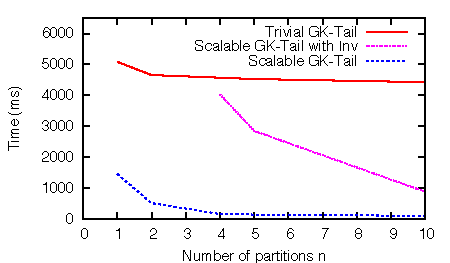
\includegraphics[width=\columnwidth]{img/perf1.pdf}}
\subfloat[]{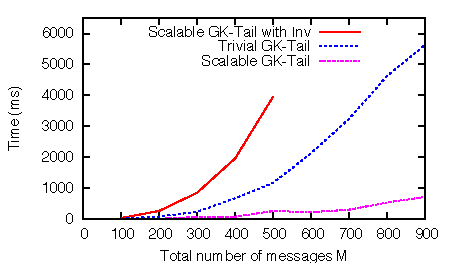
\includegraphics[width=\columnwidth]{img/perf2.pdf}}
\caption{\textbf{(a)} Trivial, Scalable, and Scalable with Invariants
  GK-Tail versions running time with M=800, r=10, k=1, and varying
  n. All algorithms benefit from a higher number of
  partitions. Scalable GK-Tail outperforms trivial
  GK-Tail. \textbf{(b)} Trivial, Scalable, and Scalable with
  Invariants GK-Tail versions running time with n=2, r=10, k=1, and
  varying M. All algorithms take longer to run on longer traces, but
  scalable GK-Tail scales much better than Trivial GK-Tail for larger
  traces. Invariants introduce a significant slowdown for large
  traces.}
\label{fig:perf1}
\end{figure*}

\begin{figure*}[!t]
\centering
\subfloat[]{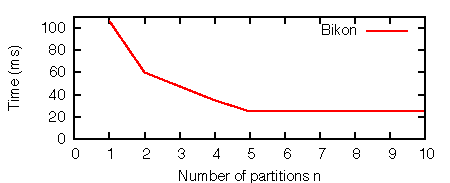
\includegraphics[width=\columnwidth]{img/perf3.pdf}}
\subfloat[]{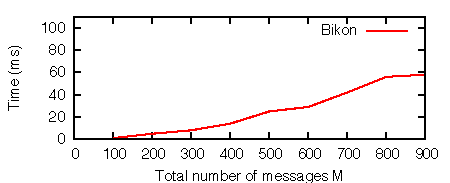
\includegraphics[width=\columnwidth]{img/perf4.pdf}}
\caption{\textbf{(a)} Bikon running time with M=800, r=10, without
  invariant inference, and with varying n. \textbf{(b)} Bikon running
  time with n=2, r=10, without invariant inference, and with varying
  M. Both graphs indicate that Bikon is much more efficient than
  GK-Tail.}
\label{fig:perf2}
\end{figure*}


% \textbf{TODO}

% reasonable properties, i.e. does a statistically significant amount of
%the observed behavior obey them, and whether they are significant
%properties, i.e. does it make sense to characterize the analyzed
%system this way.

% IB: what about utility? And who will be able to judge whether the
% characterization is 'sensical'? Depends on the person, no? I think
% we need to mention a few systems we will use: Hadoop (cite), and
% Harmony (the system that I'm working on that we can test on).  Sure
% add your stuff, and edit what is there.


% \begin{figure}[t]
%   \center {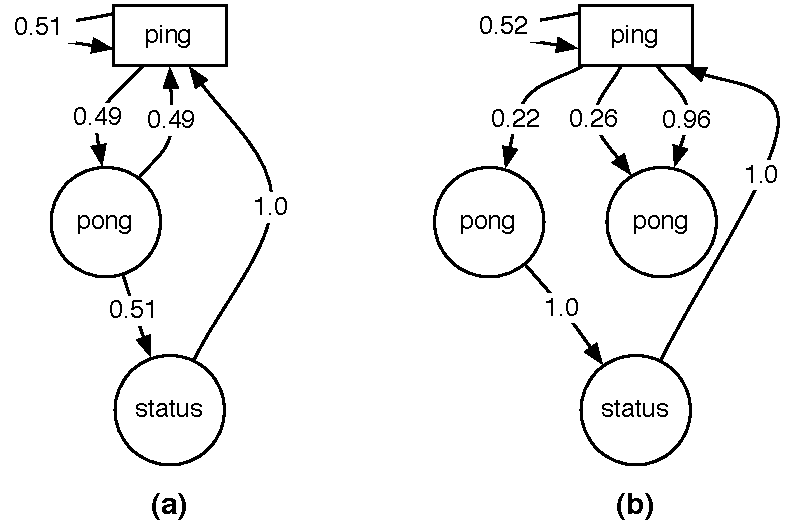
\includegraphics[scale=.6]{img/ping_pong_joined.pdf}}
%   \caption{(a) A step in the Bikon algorithm in analyzing the
%     ping-pong system (b) The next step in the Bikon algorithm that
%     partitions the pong node into two nodes, one of which always
%     transitions to a status node.}
%   \label{fig:ping_pong1}
% \end{figure}

% \caption{A sample automata representing the communication pattern in
%  the example uptime monitoring system.}

